\begin{abstract}
	In this paper we show how to use the Elliptic-curve Diffie-Hellman protocol with ephemeral keys (ECDHE) in order to share a secret message between two mobile devices by using QR codes.
	An iOS application demonstrating this approach is presented.
\end{abstract}

% ------------------------------------------------------------------------------

\section{Introduction}

Sharing secrets while an attacker is eavesdropping on the process is a problem solved a while ago.
\textcite{DBLP:journals/cacm/Merkle78} has proposed an idea that serves as a foundation for exchanging keys securely.
Modern adoptions thereof, such as the Elliptic-curve Diffie-Hellman (ECDH), are widely used in current implementations such as the TLS protocol.

Assume that two persons want to share a secret between their mobile devices without disclosing their secret to other persons looking over their shoulders.
They do not want to upload the secret to a web service, as they do not trust the service provider, and they cannot establish direct network, Bluetooth or NFC connections.
The secret could then be shared by exchanging QR codes between those devices.
Since QR codes are displayed on the device's screen, an observer could decode it.
Password protection of the shared secret is not effective, as entering the password could also be observed.
Therefore, we employ a cryptographically secure key exchange mechanism in order to protect the exchanged secret.

First, the attacker model is described.
Then the process of the protected key exchange is detailed.
In the end, an app is presented that demonstrates the described key exchange mechanism.

% ------------------------------------------------------------------------------

\section{Attacker Model}

The attacker, against whom our system is still able to protect the secret, is an outsider and has no direct access to the devices.
He could be someone, who is looking at the devices in question (shoulder surfer) or he could own surveillance cameras capturing the key exchange process.
He can capture and observe the screen of both devices at any given time.
The attacker behaves passively and only observes the key exchange process.
He is limited in his computational complexity and cannot break cryptographic systems.

% ------------------------------------------------------------------------------

\section{Process}

\begin{figure*}[t]
	\centering
	\noindent%
\begin{sequencediagram}%
	\newthread[white]{Bob}{Bob}
	\newinst[3]{Alice}{Alice}
	\begin{call}{Bob}{$K_B$}{Alice}{$K_A \concat c$}
		\begin{callself}{Alice}{}{%
			\shortstack[l]{%
				$t = k_A K_B$\\
				$k = \Function{h}{t \concat K_A \concat K_B}$\\
				$c = \Function{E}{k, m}$
			}
		}
		\end{callself}
	\end{call}
	\postlevel%
	\begin{callself}{Bob}{}{%
		\shortstack[l]{%
			$t = k_B K_A$\\
			$k = \Function{h}{t \concat K_A \concat K_B}$\\
			$m = \Function{E^{-1}}{k, c}$
		}
	}
	\end{callself}
\end{sequencediagram}

	\caption{The process of the key exchange mechanism in detail.}%
	\label{fig:key-exchange-sequence}
\end{figure*}

Assume that the two persons from the introduction are called Alice and Bob.
The Alice wants to share a secret message $m$ with Bob.
The key exchange mechanism is basically Elliptic-curve Diffie-Hellman with ephemeral keys (ECDHE)~\cite[56~pp.]{Brown:2009}.
First, both of them create ephemeral key pairs, where $k_A$ is Alice's secret and $K_A$ Alice's public key, $k_B$ and $K_B$ are Bob's keys respectively.
Bob first has to share his public key $K_B$ with Alice, so that she can determine a common session secret $t = k_A K_B = k_B K_A$ from which the actual symmetric session key $k = \Function{h}{t \concat K_B \concat K_A}$ is derived using a cryptographic hash function $h$.
Next, she sends Bob her public key $K_A$ as well as the encrypted message $c = \Function{E}{s, m}$.
Bob can now calculate the common session secret $t$ and derive the symmetric key $k$ in order to decrypt the message $m = \Function{E^{-1}}{s, c}$.
This requires two messages to be transmitted, which can be done be reading QR codes mutually from each others screens.
The process is also depicted in figure~\ref{fig:key-exchange-sequence}.

The attacker can observe both messages but can still calculate neither $t$ nor $k$ since he does know neither $k_A$ nor $k_B$.

% ------------------------------------------------------------------------------

\section{Demonstrator}

\begin{figure}[t]
	\centering
	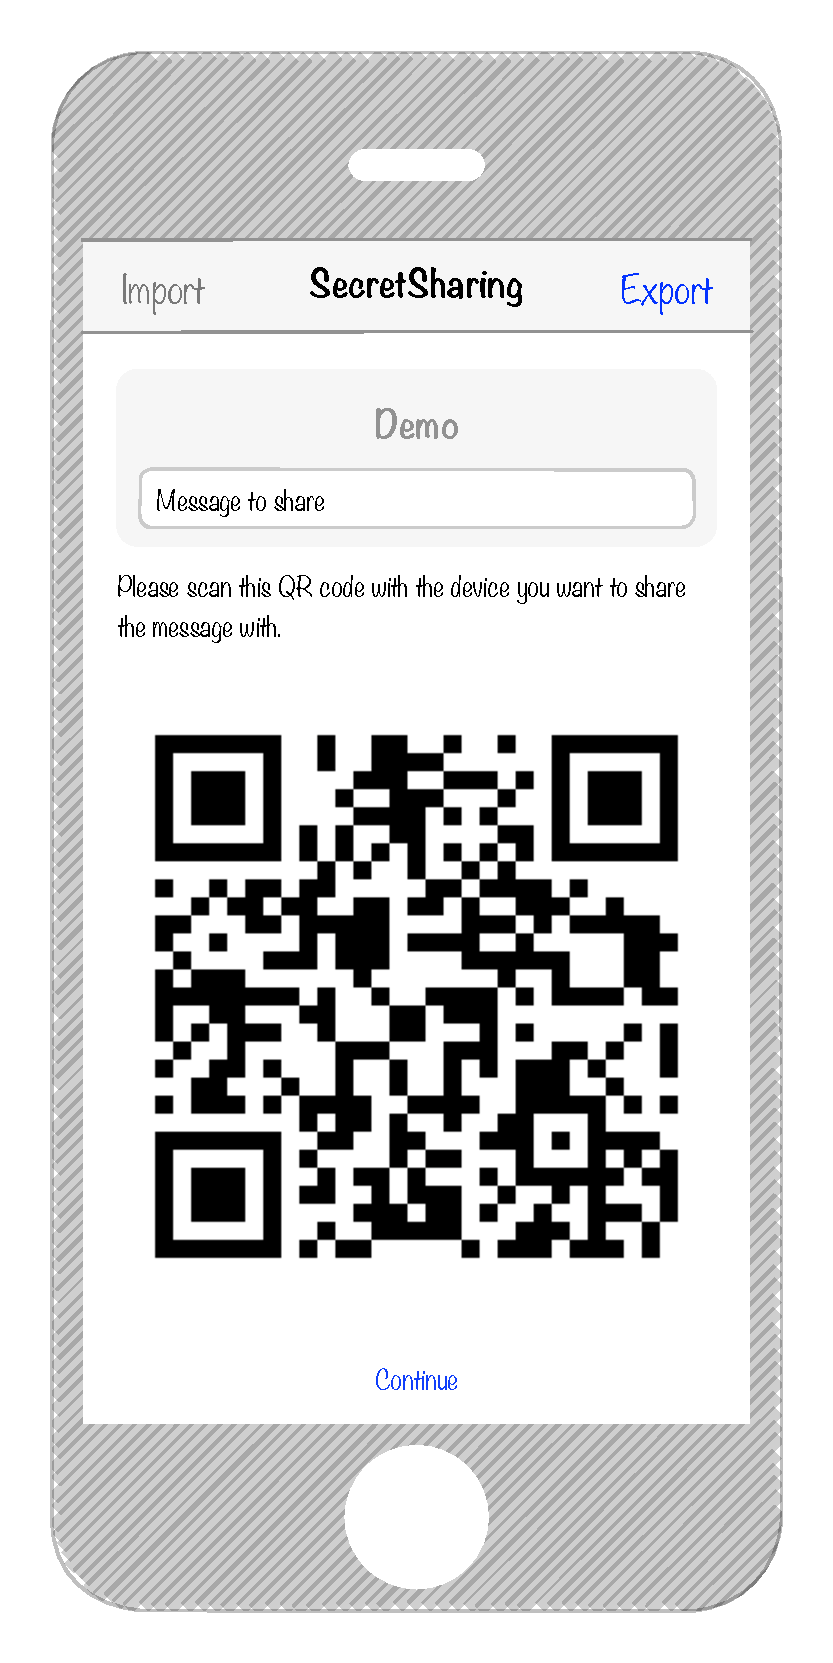
\includegraphics[width=\columnwidth]{figures/mockup.pdf}
	\caption{Mockup of the user interface of the demo application.}%
	\label{fig:mockup}
\end{figure}

In order to demonstrate this mechanism, a demo application has been designed as depicted in figure~\ref{fig:mockup}.
The application has a demonstration area, which allows the user to enter the message that should be shared with the other device.
Obviously, the demonstration area should not be present in productive apps, as the attacker would see the shared message directly.
The app works as follows:
\begin{enumerate}
	\item
		Alice enters a message on her device.
	\item
		Bob clicks \emph{Import} on his device.
		A QR code containing Bob's public key $K_B$ will be displayed there.
	\item
		Alice clicks \emph{Export} on her device.
		The camera will activate in order to scan the QR code displayed on Bob's device.
		The camera permission has to be granted for this.
		The QR code from Bob's device will automatically be detected and a QR code will be shown on Alice's device containing Alice's public key $K_A$ and the payload $c$.
	\item
		Bob clicks \emph{Continue} on his device.
		The camera will active as described for Alice's device in the previous step.
		After the QR code from Alice's device was scanned the shared message is then displayed in the demo area on Alice's device as well.
\end{enumerate}

The demo application was implemented as an open source application for iOS\footnote{AppPETs/SecretSharing-iOS: Exchange secrets between devices using QR codes: \url{https://github.com/AppPETs/SecretSharing-iOS}}.
The Sodium crypto library\footnote{The Sodium crypto library (libsodium): \url{https://libsodium.org}} library is used as implementation of the key exchange mechanism, which is using X25519~\cite{DBLP:journals/rfc/rfc7748} and Blake2b-512~\cite{Aumasson:2013, DBLP:journals/rfc/rfc7693, Aumasson:2016} internally.

% ------------------------------------------------------------------------------

\section{Limitations}

This approach might be less comfortable to users than entering a password than mutually scanning screens of two devices.
But even though the usability is impacted, it offers higher security with respect to the described attacker model.

Another limitation is that QR codes are limited in size.
This means that the shared message $m$ cannot be of arbitrary length.

The standard iOS SDK, which is used for scanning QR codes, does not support scanning QR codes in binary format, therefore the values of the QR codes are Base64 encoded.
Due to the QR code format specification, this allows slightly more data to be packed into a single QR code.

% ------------------------------------------------------------------------------

\section{Conclusion}

We presented a method for exchanging secret keys of mobile devices by mutually scanning QR codes.
The described approach uses state-of-the-art technology and protects against a passive attacker that could capture and observe the whole process.
It works without network or Bluetooth access and can be used to quickly and securely share secrets between two devices, such as exchanging addresses without the usage of a secure messenger or encrypted mail.
